% This is the HU Berlin LaTeX template, optimized for R Markdown.

% -------------------------------
% --- PREAMBLE ---
% -------------------------------
\documentclass[a4paper,11pt]{article}
\usepackage[T1]{fontenc}
\usepackage[utf8]{inputenc}
\usepackage{tgtermes}
\usepackage{amsmath,amssymb,amsfonts,amsthm}    % Typical maths resource packages
\usepackage{graphicx}                           % Packages to allow inclusion of graphics
\usepackage[bf]{caption}
\usepackage{textcomp}                           % For single quotes
\usepackage{floatrow}                           % For image and table position
\usepackage{booktabs}                           % For tables
%\usepackage[driverfallback=hypertex]{hyperref}                          
% \usepackage[bottom]{footmisc}                   
\usepackage[bottom, flushmargin]{footmisc}                   % For footnotes
\usepackage[citebordercolor={0 1 0}]{hyperref}               % For creating hyperlinks in cross references
\usepackage{footnotebackref}
\usepackage{setspace}

% -------------------------------
% --- some layout definitions ---
% -------------------------------

% define topline
\usepackage[automark]{scrlayer-scrpage}
\pagestyle{scrheadings}
\automark{section}
\clearscrheadings
\ohead{\headmark}




% define page size, margin size
\setlength{\headheight}{1.1\baselineskip}
\voffset=-2cm
\hoffset=-3cm
\textheight24cm
\textwidth15.5cm
\topmargin1cm
\oddsidemargin3cm
\evensidemargin3cm
\setcounter{secnumdepth}{3}
\setcounter{tocdepth}{3}   
  \usepackage[parfill]{parskip} 

% define line spacing = 1.5
\renewcommand{\baselinestretch}{1.5}

% define position of graphics
\floatsetup[figure]{capposition=bottom}
\floatsetup[table]{capposition=bottom}
\floatplacement{figure}{ht}
\floatplacement{table}{ht}

% save thesis parameters for later
\newcommand{\thesistype}{Master's Thesis}
\newcommand{\thesisauthor}{Elias Cuadra Braatz}
\newcommand{\thesisdate}{July 01, 2021}

% define tightlist to work with newer versions of pandoc
\providecommand{\tightlist}{%
  \setlength{\itemsep}{0pt}\setlength{\parskip}{0pt}}

% change spacing
\setlength {\parskip}{1em}

% Additional LaTeX parameters added in the YAML header of index.Rmd


%fix csl issue
\newlength{\cslhangindent}
\setlength{\cslhangindent}{1.5em}
\newlength{\csllabelwidth}
\setlength{\csllabelwidth}{3em}
\newenvironment{CSLReferences}[3] % #1 hanging-ident, #2 entry spacing
 {% don't indent paragraphs
  \setlength{\parindent}{0pt}
  % turn on hanging indent if param 1 is 1
  \ifodd #1 \everypar{\setlength{\hangindent}{\cslhangindent}}\ignorespaces\fi
  % set entry spacing
  \ifnum #2 > 0
  \setlength{\parskip}{#2\baselineskip}
  \fi
 }%
 {}
\usepackage{calc} % for \widthof, \maxof
\newcommand{\CSLBlock}[1]{#1\hfill\break}
\newcommand{\CSLLeftMargin}[1]{\parbox[t]{\maxof{\widthof{#1}}{\csllabelwidth}}{#1}}
\newcommand{\CSLRightInline}[1]{\parbox[t]{\linewidth}{#1}}
\newcommand{\CSLIndent}[1]{\hspace{\cslhangindent}#1}




% --------------------------------------
% --------------------------------------
% --------------------------------------
% --- the structure the tex document ---
% ---  (this our recommendation) -------
% frontmatter:
%   - titlepage (mandatory),
%   - acknowledgement,
%   - abstract,
%   - table of contents (mandatory),
%   - list of abbreviations (not mandatory),
%   - list of figures (not mandatory),
%   - list of tables  (not mandatory) .
%
% body of the thesis (the structure of the thesis body is not mandatory, but the list of literature is mandatory):
%   - introduction,
%   - methods,
%   - data,
%   - results,
%   - conclusion,
%   - literature (mandatory),
%   - appendix (figures, tables).
%
% last page:
%   - declaration of authorship (mandatory).
% --------------------------------------
% --------------------------------------
% --------------------------------------
\begin{document}

% -------------------------------
% --- frontmatter: Title page ---
% -------------------------------
\thispagestyle{empty}
\begin{center}
  \vspace*{5mm}
  \linespread{1.5}
  {\huge{\bf Windenergy and repowering potential in Rhineland-Palatinate from 2021 until 2030}\par}\vspace{1cm}
  Master's Thesis submitted \\\vspace{0.5cm}
  to \\\vspace{0.5cm}
  \textbf{Dr.~Stefan Jergentz} \\
  \textbf{Dr.~Nanki Sidhu} \\\vspace{1.5cm}
  
  
  
\includegraphics[width=0.5\textwidth]{Uni-Logo-2.jpg}
  
  Institute of Environmental Sciences \\
  Environmental Economics \\
   Chair: Prof.~Oliver Frör \\  \vspace{1cm}

  
  
  by \\\vspace{0.5cm}
  \textbf{Elias Cuadra Braatz} \\
  (219202265) \\
  
  \medskip
  \medskip
  in partial fulfillment of the requirements \\
  for the degree of \\
  \textbf{Master of Environmental Sciences} \\\vspace{0.5cm}
  July 01, 2021
  
\end{center}


% -----------------------------
% --- frontmatter: Contents ---
% -----------------------------
\newpage
\tableofcontents
\clearpage

% -----------------------------
% --- frontmatter: Abstract ---
% -----------------------------
\newpage
\hypertarget{abstract}{%
\section*{Abstract}\label{abstract}}
\addcontentsline{toc}{section}{Abstract}

This is the template for a thesis at the Chair of Econometrics of
Humboldt--Universit"at zu Berlin. A popular approach to write a thesis or a
paper is the IMRAD method (Introduction, Methods, Results and Discussion). This
approach is not mandatory! You can find more information about formal
requirements in the booklet `Hinweise zur Gestaltung der äußeren Form von
Diplomarbeiten' which is available in the office of studies.

The abstract should not be longer than a paragraph of around 10-15 lines (or
about 150 words). The abstract should contain a concise description of the
econometric/economic problem you analyze and of your results. This allows the
busy reader to obtain quickly a clear idea of the thesis content.

% ----------------------------------------------------------
% --- frontmatter: List of Abbreviations (not mandatory) ---
% ----------------------------------------------------------
\newpage
\hypertarget{list-of-abbreviations}{%
\section*{List of Abbreviations}\label{list-of-abbreviations}}
\addcontentsline{toc}{section}{List of Abbreviations}
\begin{tabular}{rp{0.2cm}lp{1cm}rp{0.2cm}l}
    CPI     & &  Consumer Price Index   & & ETF     & &  Equity Traded Funds  \\
    ETH     & &  Eat the Horse          & & XLM     & &  Xetra Liquidity
\end{tabular}
% ----------------------------------------------------
% --- frontmatter: List of Figures (not mandatory) ---
% ----------------------------------------------------
\newpage
\listoffigures
\addcontentsline{toc}{section}{List of Figures}

% ---------------------------------------------------
% --- frontmatter: List of Tables (not mandatory) ---
% ---------------------------------------------------
\newpage
\listoftables
\addcontentsline{toc}{section}{List of Tables}

% -------------------------------
% --- main body of the thesis ---
% -------------------------------
\newpage
\pagestyle{plain}       
\setcounter{page}{1}    % start page numbering anew
\pagenumbering{arabic}  % page numbers in arabic style

\hypertarget{introduction}{%
\section{Introduction}\label{introduction}}

This work was executed and written in scientific recognition of the importance of reducing greenhouse gas emissions and expanding renewable energies to mitigate the effects of climate change.
This study was also carried out on behalf of the state-owned energy agency {[}\protect\hyperlink{ref-EnergieagenturRheinlandPfalz.2021}{1}{]} within the project ``municipal greenhouse gas accounting and regional climate protection portals in Rhineland-Palatinate'' {[}\protect\hyperlink{ref-KomBiReK.2021}{2}{]} which is funded by the ``European Regional Development Fund'' {[}\protect\hyperlink{ref-EuropeanRegionalDevelopmentFund.2021}{3}{]} and the state of Rhineland-Palatinate. This project supports the creation of municipal climate protection measures in order to achieve the climate protection goals of the municipalities and the state and thereby increases regional added value, ensures sustainability and thus improves the quality of life of all citizens. When developing municipal climate protection, a sound strategy is required regarding the legally anchored striving for climate neutrality of the state of Rhineland-Palatinate (Landesklimaschutzgesetz §4, 2014, {[}\protect\hyperlink{ref-RheinlandPfalz.19.08.2014}{4}{]}). Even more pressure comes from the recent press release No.~31/2021 of April 29 in 2021 {[}\protect\hyperlink{ref-Bundesverfassungsgericht.24.03.2021}{5}{]}, in which the first Senate of the Federal Constitutional Court decided that the regulations of the Climate Protection Act of December 12 in 2019 {[}KSG, 2019{]} on the national climate protection targets and the annual emission quantities permitted up to 2030 are incompatible with fundamental rights, as there are no sufficient criteria for further emission reductions from 2031 onwards. It is stated that the legal requirements are not sufficient to bring about a timely transition to climate neutrality. The legislature has therefore published an adjusted edition of this act that strives for a faster development of renewable energies and the energy transition in general {[}\protect\hyperlink{ref-BundesministeriumfurUmweltNaturschutzundnukleareSicherheit.12.05.2021}{6}{]}. This shows that this study is also highly embedded in a socio-economic context.
The energy transition is a cornerstone of a decent strategy to climate neutrality and Rhineland-Palatinate wants to play a pioneering role in the implementation of the energy transition. The state government publishes on its website that Rhineland-Palatinate will cover 100 \% of its electricity needs from renewable energies by 2030. In addition to energy from the sun, water and biomass, two thirds of the electricity generated in 2030 should come from wind power and is therefore the subject of this master thesis {[}\protect\hyperlink{ref-LandesregierungRheinlandPfalz.2021}{7}{]}.
The gross electricity generation in Rhineland-Palatinate from wind power rose in 2017 with 5.9 TWh to 29 \% of the total 20.7 TWh generated electricity. The total consumption in the same year was 29.1 TWh {[}\protect\hyperlink{ref-Lehnert.2020}{8}{]}. It can be assumed that, on the one hand, electricity consumption will increase in the future due to the electrification of transport and domestic heating, and on the other hand, efficiency measures can also lead to a lower energy consumption. Various scenarios about future electricity consumption assume a slightly reduced to increased, but on average relatively unchanged electricity consumption for the whole of Germany in 2030 {[}\protect\hyperlink{ref-NormanGerhardt.2015}{9}{]}. In order to achieve the self-set goals of using two thirds of the electricity demand from wind power with constant or higher electricity demand, electricity generation with wind turbines (WT's) must be increased to at least 14 TWh per year. If Rhineland-Palatinate wants to become independent of electricity imports, an increase to around 20 TWh is necessary. There are two ways of increasing the amount of electricity generated by wind energy. On the one hand, areas that are still available can be identified and built on with new WPP's. On the other hand, existing old systems, whose absolute electricity feed-in quantity is low, can be replaced by new, higher and more efficient systems through the so-called ``repowering.''
The aim of this work is to develop a methodology for calculating the wind energy potential and its related area consumption at the state level as well as for the districts and association communities in Rhineland-Palatinate. With this results an evaluation of the desired expansion targets should be assessed. The central three questions of this work are therefore:
\begin{enumerate}
\def\labelenumi{\arabic{enumi}.}
\item
  How much electric energy can be generated by a new wind turbine from 2021 until 2030 in Rhineland-Palatinate per area?
\item
  How large is the potential when all wind turbines with a commissioning date before 2005 are repowered?
\item
  How much area is needed to generate the target amount of 20 TWh out of wind energy?
\end{enumerate}
In order to answer these questions, the technical fundamentals of the electricity yield from WT's are explained first. Subsequently, the master and movement data provided by the transmission system operator Amprion, which document all electricity fed into the public grid by WT's and other technical information, is analysed and a forecasted up to the year 2030. The respective area consumption to generate that electricity is calculated using a GIS based approach. As a by-product the greenhouse gas reduction potential can be derived from the potential for electricity generation. Knowing the electricity potential per area, the required area for the generation targets can be calculated and an assessment of the given expectations can be made subsequently.

\hypertarget{state-of-the-art}{%
\section{State of the art}\label{state-of-the-art}}

\hypertarget{technical-and-physical-basics}{%
\subsection{Technical and physical basics}\label{technical-and-physical-basics}}

Wind energy has been used by humans for thousands of years, but the generation of electrical power has only been possible since the 19th century with the beginning of industrialization and is now the subject of constant research and development in the context of the energy transition {[}\protect\hyperlink{ref-Wikipedia.2021}{10}{]}. A wind turbine usually consists of the three main components rotor blades, nacelle and tower. The nacelle contains besides other elements the gearbox, the generator, the transformer and the control system {[}\protect\hyperlink{ref-MladenBosnjakovic.2013}{11}{]}. The mostly three rotor blades are attached to the rotor hub and absorb the kinetic energy of the wind and convert it into a rotary motion. If the winds are too strong, the rotor blades can be ``taken out of the wind'' by adjusting the blades, thus protecting the system from damage. Mainly the gearbox and the generator convert the kinetic energy into electricity. However, there are also systems with direct drive and without gear. The nacelle can be rotated to an optimal position when the wind conditions change, and an electromagnetic brake helps to shut down the system when the winds are too strong or during maintenance work. In addition to its load-bearing function, the tower also contains the power lines that conduct electricity to the grid connection of the distribution network {[}\protect\hyperlink{ref-NetzKonstrukteur.16.11.2020}{12}{]}.

The transmission system operators, in this case Amprion, are obliged to publish master and so-called movement data for each calendar year in accordance with section 77 Renewable Energy Act 2017. These movement data include the annual electricity generation and the underlying tariff for each renewable energy system. The movement data for Rhineland-Palatinate are currently available until 2019. The total amount of electricity fed in with remuneration in 2019 from wind turbines in RLP is 6,782,180,753 kWh, i.e.~approx. 6,782 TWh {[}\protect\hyperlink{ref-EnergieagenturRheinlandPfalz.2019}{13}{]}.

The amount of electricity generated by a wind turbine, the electricity yield, can be derived from the physical relationship between the kinetic energy and the power of the wind. Without claiming to be exhaustive, the following applies\footnote{\(E_{kin}= kinetic\; energy,\; m=mass\; of\; air,\; v= wind\;speed\)}:
\begin{equation}
E_{kin} = \frac{1}{2}mv^2
\end{equation}
The air throughput or mass flow \(\hat{m}\) that flows through the area swept by the rotor blades in a certain time can be calculated by multiplying the air density, rotor area and wind speed as well as the time interval required with\footnote{\(\rho= density\; of\; air,\; A= rotor\; area\)}:
\begin{equation}
\hat{m}=\rho A V
\end{equation}
The power P is equal to the energy per unit of time \(\hat{E}\). This results in the power of the wind with\footnote{\(r= radius\; of\; rotor\)}:
\begin{equation}
P_{wind}=\hat{E}=\frac{1}{2}\hat{m}v^2=\frac{1}{2} \rho \pi r^2 v^3
\end{equation}
(Mac Kay {[}ref{]} and BWE {[}ref{]})

Of course, not all the wind's power can be converted and there are further losses when converting kinetic energy into electrical energy in the generator. The efficiency in theory is a maximum of 59\% and in practice it is often around 40 \% to a maximum of 50 \% {[}reference{]}. In Formula 3, however, it becomes clear that the wind speed is the decisive factor for the performance of the wind and thus a wind turbine. If the wind speed increases three times, the power is 27 times greater. It can also be seen that the amount of energy increases proportionally with increasing rotor diameter. This explains why the rotor diameters become larger in practice. Due to the higher and more constant wind speed with increasing height, the hub heights also increase. The development of the rotor diameter and hub heights are shown in figures \ref{fig:rotor} and \ref{fig:nabe}. For the classification of the technical development and the calculation method, the study of the German Wind Guard (DWG) ``Full load hours of wind turbines on land - development, influences, effects'' from October 5th, 2020 {[}reference{]}, is used as a guide and its results are presented. The study examines the development of the full load hours and thus also the wind energy potential in Germany and is divided into the sub-areas Schleswig-Holstein (SH), north (Norden), centre (Mitte) and south (Süden). Rhineland-Palatinate is part of the southern region.
\begin{figure}

{\centering 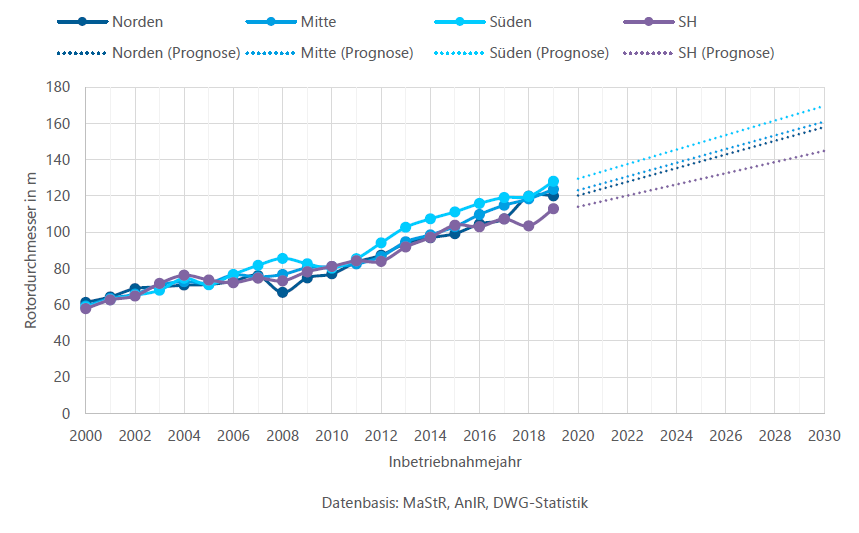
\includegraphics[width=1\linewidth]{figures/DWG/DWG_Rotordurchmesser} 

}

\caption{Development and forecast of the mean rotor diameter according to Deutsche WindGuard, 2020}\label{fig:rotor}
\end{figure}
\begin{figure}

{\centering \includegraphics[width=1\linewidth]{figures/DWG/DWG_Nabenhöhe} 

}

\caption{Development and forecast of mean hub hight according to Deutsche WindGuard, 2020}\label{fig:nabe}
\end{figure}
The study of DWG suggests that the wind energy potential, i.e.~the theoretical electricity yield of a wind turbine for future systems, can and will be calculated in this work using the following formula:
\[
Electricity\;yield\; =\; Full\;load\;hours\; *\; Capacity
\]
The capacity is the installed nominal output, also called \textbf{rated capacity} of the generator and can be found in the technical details of a wind turbine generator. The development of the installed nominal power depending on the commissioning date in Germany can be seen in figure \ref{fig:capacity}.
\begin{figure}

{\centering 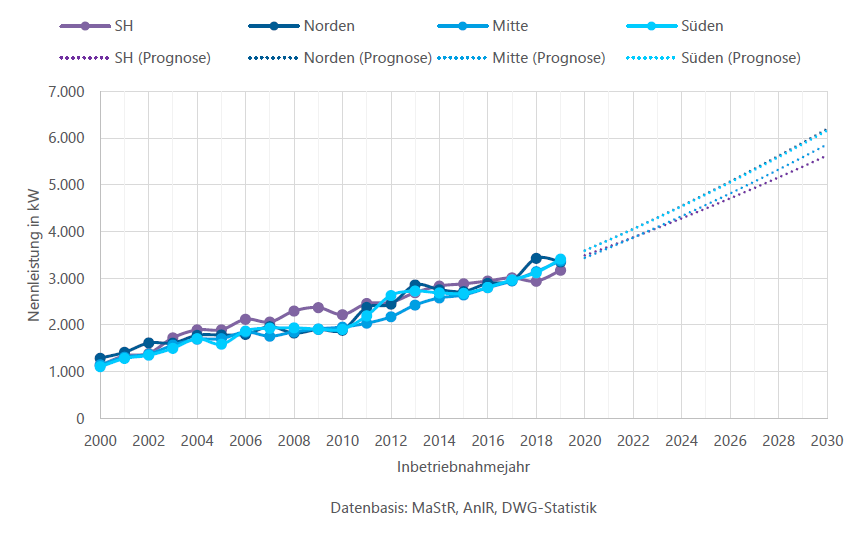
\includegraphics[width=1\linewidth]{figures/DWG/DWG_Nennleistung} 

}

\caption{Development and forecast of the mean rated capacity according to Deutsche WindGuard, 2020}\label{fig:capacity}
\end{figure}
The \textbf{full load hours} are formed from the quotient of the annual electricity yield and the rated capacity and are an indicator of the degree of utilization of a wind turbine. The full load hours number the hours that the system would have to be operated under nominal load in order to deliver the amount of electricity generated and do not reflect the actual operating time below nominal load. Since the full load hours result from the electricity yield and the installed nominal power, there is a dependency and the gain in information is limited. However, the full load hours are a useful concept in order to be able to draw conclusions about the electricity yield and, therefore, analysis of the full load hours of Rhineland-Palatinate are presented in Section 3.2.3. The development of full load hours in Germany can be seen in figure \ref{fig:flh}.
\begin{figure}

{\centering 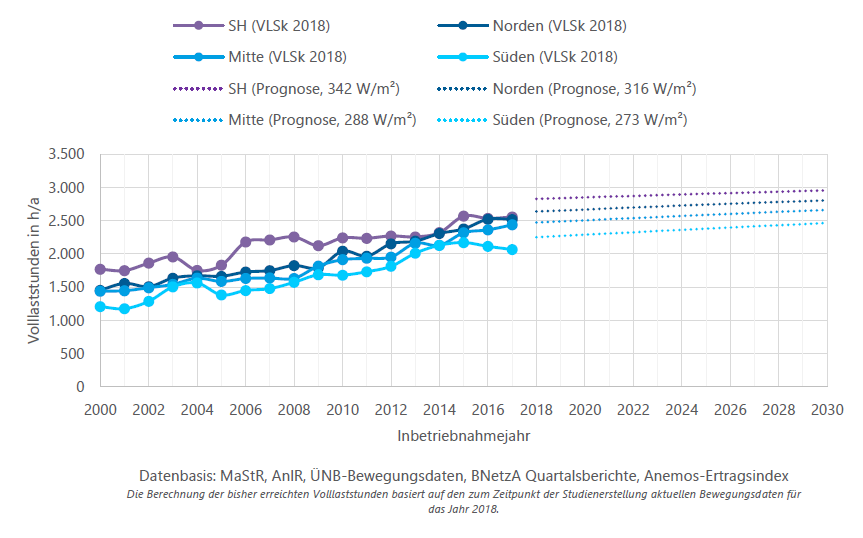
\includegraphics[width=1\linewidth]{figures/DWG/DWG_Volllaststunden} 

}

\caption{Development and forecast of the mean full load hours according to Deutsche WindGuard, 2020}\label{fig:flh}
\end{figure}
If two plants have the same hub height and the same rotor diameter, but a different nominal power, the less powerful plant, i.e.~the plant with the lower \textbf{specific nominal power}, will achieve more full-load hours but a lower annual energy yield at the same wind speeds. The full load hourly value should therefore always be considered and evaluated in connection with the energy yield.The specific nominal power represents the relationship between the nominal power of the turbine and the swept rotor area. The specific nominal power of the turbines has tended to decrease since 2012, which is due to the increasing rotor diameters figure \ref{fig:rotor}. Systems with a lower specific nominal output, i.e.~comparatively larger rotors, have more full-load hours under the same wind conditions or achieve their nominal output at lower wind speeds and are therefore also referred to as low-wind systems. If you compare two systems with the same rotor diameter, the system with a higher absolute and therefore also specific nominal output is always more expensive and is therefore only suitable for comparatively higher wind speeds. Due to the prevailing conditions in Rhineland-Palatinate, low-wind turbines with a lower specific nominal output are more important in repowering than the increase in absolute turbine output. However, the value of the specific nominal output in southern Germany is currently stagnating at approx. 270 W / m² (Figure 5).

\newpage

\hypertarget{data}{%
\section{Data}\label{data}}
\begin{itemize}
\item
  Describe the data and its quality.
\item
  How was the data sample selected?
\item
  Provide descriptive statistics such as:
  \begin{itemize}
  \item
    time period,
  \item
    item number of observations, data frequency,
  \item
    item mean, median,
  \item
    item min, max, standard deviation,
  \item
    item skewness, kurtosis, Jarque--Bera statistic,
  \item
    item time series plots, histogram.
  \end{itemize}
\item
  For example:
\end{itemize}
\begin{table}[H]

\caption{\label{tab:table1}Detailed descriptive statistics of location and dispersion for 2100 observed swap rates for the period from February 15, 1999 to March 2, 2007. Swap rates measured as 3.12 (instead of 0.0312).}
\centering
\begin{tabular}[t]{lrrrrrrrrrr}
\toprule
  & 3m & 6m & 1yr & 2yr & 3yr & 5yr & 7yr & 10yr & 12yr & 15yr\\
\midrule
Mean & 3.138 & 3.191 & 3.307 & 3.544 & 3.756 & 4.093 & 4.354 & 4.621 & 4.741 & 4.878\\
StD & 0.915 & 0.919 & 0.935 & 0.910 & 0.876 & 0.825 & 0.803 & 0.776 & 0.768 & 0.762\\
\midrule
\bottomrule
\end{tabular}
\end{table}
\begin{itemize}
\item
  Allows the reader to judge whether the sample is biased or to evaluate
  possible impacts of outliers, for example.
\item
  Here tables can be easily integrated using the \texttt{kable()} function in the
  \texttt{knitr} package (with perhaps some additional help from the \texttt{kableExtra}
  package). \texttt{kable()} will automatically generate a label for the table
  environment. That way you don't have to manually enter in the table in LaTex,
  you can embed tables from R code.
\item
  Tables can be referenced using \texttt{\textbackslash{}@ref(label)}, where \texttt{label} is \texttt{tab:\textless{}name\textgreater{}},
  where \texttt{\textless{}name\textgreater{}} is the code chunk label.
\item
  The appearance may look different to tables directly typed with LaTex, due to
  limitations in \texttt{kable()}. To compare:
  \begin{table}[ht]
    \begin{center}
        {\footnotesize
        \begin{tabular}{l|cccccccccc}
            \hline \hline
                      & 3m    & 6m    & 1yr   & 2yr   & 3yr   & 5yr   & 7yr   & 10yr  & 12yr  & 15yr   \\
            \hline
                Mean   & 3.138 & 3.191 & 3.307 & 3.544 & 3.756 & 4.093 & 4.354 & 4.621 & 4.741 & 4.878  \\
                StD    & 0.915 & 0.919 & 0.935 & 0.910 & 0.876 & 0.825 & 0.803 & 0.776 & 0.768 & 0.762  \\
            \hline \hline
        \end{tabular}}
    \end{center}
    \caption{This table was handwritten with LaTeX.}
    \label{tab:table2}
    \end{table}
\end{itemize}
\hypertarget{results}{%
\section{Results}\label{results}}

\hypertarget{conclusion}{%
\section{Conclusion}\label{conclusion}}
\begin{itemize}
\item
  Give a short summary of what has been done and what has been found.
\item
  Expose results concisely.
\item
  Draw conclusions about the problem studied. What are the implications of your
  findings?
\item
  Point out some limitations of study (assist reader in judging validity of
  findings).
\item
  Suggest issues for future research.
\end{itemize}
\newpage

\hypertarget{references}{%
\section*{References}\label{references}}
\addcontentsline{toc}{section}{References}

\noindent

\setlength{\parindent}{-0.5cm}
\setlength{\leftskip}{0.5cm}
\setlength{\parskip}{8pt}

\hypertarget{refs}{}
\begin{CSLReferences}{0}{0}
\leavevmode\hypertarget{ref-EnergieagenturRheinlandPfalz.2021}{}%
\CSLLeftMargin{1. }
\CSLRightInline{Energieagentur Rheinland-Pfalz: \url{https://www.energieagentur.rlp.de/}, (2021)}

\leavevmode\hypertarget{ref-KomBiReK.2021}{}%
\CSLLeftMargin{2. }
\CSLRightInline{KomBiReK: Kommunale treibhausgas-bilanzierung und regionale klimaschutzportale rheinland-pfalz, \url{https://www.energieagentur.rlp.de/projekte/kommune/kombirek}, (2021)}

\leavevmode\hypertarget{ref-EuropeanRegionalDevelopmentFund.2021}{}%
\CSLLeftMargin{3. }
\CSLRightInline{European Regional Development Fund: \url{https://ec.europa.eu/regional_policy/de/funding/erdf/}, (2021)}

\leavevmode\hypertarget{ref-RheinlandPfalz.19.08.2014}{}%
\CSLLeftMargin{4. }
\CSLRightInline{Rheinland-Pfalz: Landesgesetz zur f{ö}rderung des klimaschutzes - landesklimaschutzgesetz: LKSG, \url{http://landesrecht.rlp.de/jportal/portal/t/onc/page/bsrlpprod.psml?pid=Dokumentanzeige\&showdoccase=1\&js_peid=Trefferliste\&documentnumber=1\&numberofresults=22\&fromdoctodoc=yes\&doc.id=jlr-KlimaSchGRPrahmen\&doc.part=X\&doc.price=0.0\&doc.hl=1}, 19.08.2014}

\leavevmode\hypertarget{ref-Bundesverfassungsgericht.24.03.2021}{}%
\CSLLeftMargin{5. }
\CSLRightInline{Bundesverfassungsgericht: Verfassungsbeschwerden gegen das klimaschutzgesetz teilweise erfolgreich: Pressemitteilung nr. 31/2021 vom 29. April 2021, \url{https://www.bundesverfassungsgericht.de/SharedDocs/Pressemitteilungen/DE/2021/bvg21-031.html}, 24.03.2021}

\leavevmode\hypertarget{ref-BundesministeriumfurUmweltNaturschutzundnukleareSicherheit.12.05.2021}{}%
\CSLLeftMargin{6. }
\CSLRightInline{Bundesministerium für Umwelt, Naturschutz und nukleare Sicherheit: Entwurf eines ersten gesetzes zur {Ä}nderung des bundes-klimaschutzgesetzes, \url{https://www.bmu.de/gesetz/952/}, 12.05.2021}

\leavevmode\hypertarget{ref-LandesregierungRheinlandPfalz.2021}{}%
\CSLLeftMargin{7. }
\CSLRightInline{Landesregierung Rheinland-Pfalz: Wind, sonne, wasser: Ausbau der erneuerbaren energien in der stromerzeugung, \url{https://www.rlp.de/de/regierung/schwerpunkte/energiewende/\#:~:text=Rheinland\%2DPfalz\%20wird\%20bis\%20zum,einem\%20Viertel\%20entfallen}, (2021)}

\leavevmode\hypertarget{ref-Lehnert.2020}{}%
\CSLLeftMargin{8. }
\CSLRightInline{Dr. N. M. Lehnert und M. Herzig: Statistische monatshefte rheinland-pfalz: Strommix und energieverbrauch in rheinland-pfalz, \url{https://www.statistik.rlp.de/fileadmin/dokumente/monatshefte/2020/April/04-2020-225.pdf}, (2020)}

\leavevmode\hypertarget{ref-NormanGerhardt.2015}{}%
\CSLLeftMargin{9. }
\CSLRightInline{Norman Gerhardt, F.S.: Fraunhofer IWES (2015): Wie hoch ist der stromverbrauch in der energiewende? Energiepolitische zielszenarien 2050 -- r{ü}ckwirkungen auf den ausbaubedarf von windenergie und photovoltaik: Studie im auftrag von agora energiewende. 086/19-S-2015/DE, (2015)}

\leavevmode\hypertarget{ref-Wikipedia.2021}{}%
\CSLLeftMargin{10. }
\CSLRightInline{Wikipedia: Geschichte der windenergie, \url{https://de.wikipedia.org/wiki/Geschichte_der_Windenergienutzung}, (2021)}

\leavevmode\hypertarget{ref-MladenBosnjakovic.2013}{}%
\CSLLeftMargin{11. }
\CSLRightInline{Mladen Bošnjaković: Wind energy technology trends: Conference paper, \url{https://www.researchgate.net/publication/310766589_WIND_ENERGY_TECHNOLOGY_TRENDS}, (2013)}

\leavevmode\hypertarget{ref-NetzKonstrukteur.16.11.2020}{}%
\CSLLeftMargin{12. }
\CSLRightInline{NetzKonstrukteur: Wie funktioniert eine windkraftanlage? Aufbau einer windkraftanlage, \url{https://netzkonstrukteur.de/wie-funktioniert-eine-windkraftanlage/}, 16.11.2020}

\leavevmode\hypertarget{ref-EnergieagenturRheinlandPfalz.2019}{}%
\CSLLeftMargin{13. }
\CSLRightInline{EEG-StammBew{\_}2019{\_}amprion-EAtlas.xlsx /master and movement data from amprion of the year 2019 preprocessed through the energy agency of rhineland-palatinate - the file and the code with which the data was further processed comes with this document., (2019)}

\end{CSLReferences}
\indent
\setlength{\parindent}{17pt}
\setlength{\leftskip}{0pt}
\setlength{\parskip}{0pt}

\newpage

\appendix

\hypertarget{appendix}{%
\section{Appendix}\label{appendix}}

Here goes the appendix!

\hypertarget{figures}{%
\subsection{Figures}\label{figures}}

\hypertarget{tables}{%
\subsection{Tables}\label{tables}}
\begin{table}[ht]
    \begin{center}
        {\footnotesize
        \begin{tabular}{l|cccccccccc}
        \hline \hline
                        & 3m    & 6m    & 1yr   & 2yr   & 3yr   & 5yr   & 7yr   & 10yr  & 12yr  & 15yr   \\
            \hline
                Mean   & 3.138 & 3.191 & 3.307 & 3.544 & 3.756 & 4.093 & 4.354 & 4.621 & 4.741 & 4.878  \\
                Median & 3.013 & 3.109 & 3.228 & 3.490 & 3.680 & 3.906 & 4.117 & 4.420 & 4.575 & 4.759  \\
                Min    & 1.984 & 1.950 & 1.956 & 2.010 & 2.240 & 2.615 & 2.850 & 3.120 & 3.250 & 3.395  \\
                Max    & 5.211 & 5.274 & 5.415 & 5.583 & 5.698 & 5.805 & 5.900 & 6.031 & 6.150 & 6.295  \\
                StD    & 0.915 & 0.919 & 0.935 & 0.910 & 0.876 & 0.825 & 0.803 & 0.776 & 0.768 & 0.762  \\
            \hline \hline
        \end{tabular}}
    \end{center}
    \caption{Detailed descriptive statistics of location and dispersion for
    2100 observed swap rates for the period from
    February 15, 1999 to March 2, 2007. Swap rates measured as 3.12 (instead of 0.0312).}
    \label{tab:apptable}
\end{table}
\newpage

% change rmd_files in `_bookdown.yml` files to determine order
% note that references and appendix are also contained here.



% --------------------------------------------
% --- last page: Declaration of Authorship ---
% --------------------------------------------

\newpage
\thispagestyle{empty}
\hypertarget{declaration-of-authorship}{%
\section*{Declaration of Authorship}\label{declaration-of-authorship}}

I hereby confirm that I have authored this \thesistype{} independently and
without use of others than the indicated sources. All passages which are
literally or in general matter taken out of publications or other sources are
marked as such.
\vspace{1cm}

Berlin, \thesisdate{}
\vspace{3cm}

. . . . . . . . . . . . . . . . . . . . . . . . . . . . . . .
\vspace{0.1cm}

\thesisauthor{}


\end{document}
